\label{sec:method}
We aim to extend the limits of off-policy in-context RL's three main barriers: 1) the memory limit or context length $l$, 2) the value discount factor $\gamma$, and 3) the size and recall of our sequence model. Transformers are a strong solution to the last challenge and may be able to address all three barriers if we were able to learn from long context lengths $l \approx H$ and select actions for $\gamma \geq .999$ at test time. In principle, this would allow agents to remember and plan for long adaptation windows in order to scale to more challenging problems while removing the need to tune trade-offs between stability and context length. AMAGO overcomes several challenges to make this possible. This section summarizes the most important techniques that enable AMAGO's performance and flexibility. More details can be found in Appendix \ref{app:implementation_details} and in our open-source code release.

A high-level overview of AMAGO is illustrated in Figure \ref{fig:amago}. The observations of every environment are augmented to a unified goal-conditioned CMDP format, even when some of the extra input information is unnecessary. This unified format allows AMAGO to be equally applicable to generalization, meta-RL, long-term memory, and multi-task problems without changes. AMAGO is an off-policy method that takes advantage of large and diverse datasets; trajectory data is loaded from disk and can be relabeled with alternative goals and rewards. The shape and format of trajectories vary across domains, but we use a timestep encoder network to map each timestep to a fixed-size representation. AMAGO allows the timestep encoder to be the only architecture change across experiments. A single Transformer trajectory encoder processes sequences of timestep representations. AMAGO uses these representations as the inputs to small feed-forward actor and critic networks, which are optimized simultaneously across every timestep of the causal sequence. Like all implicit context-based methods (Sec. \ref{sec:related}), this architecture encourages the trajectory encoder outputs to be latent estimates of the current state and environment $(s_i, e)$ (Sec. \ref{sec:background}). In short, AMAGO's learning update looks more like supervised sequence modeling than an off-policy actor-critic, where each training step involves exactly one forward pass of one Transformer model with two output heads. This end result is simple and scalable but is only made possible by important technical details. 

\paragraph{Sharing One Sequence Model.} The accepted best practice in off-policy RL is to optimize separate sequence models for the actor and critic(s) --- using additional target models to compute the critic loss. Sharing actor and critic sequence models is possible but has repeatedly been shown to be unstable \cite{ni2022recurrent, yang2021recurrent, yarats2021improving}. AMAGO addresses this instability and restructures the learning update to train its actor and critics on top of the same sequence representation; there are no target sequence models, and every parameter is updated simultaneously without alternating steps or conflicting learning rates. We combine the actor and critic objectives into a single loss trained by one optimizer. However, we must put each term on a predictable scale to prevent their weights from needing to be tuned across every experiment \cite{van2016learning, hafner2020mastering}. The key detail enabling the simultaneous update to work in AMAGO --- without separating the Transformer from the actor loss \cite{yarats2021improving, yang2021recurrent} --- is to carefully detach the critic from the actor loss (Appendix \ref{app:shared_update}). We compute loss terms with a custom variant of REDQ \cite{chen2021randomized} for discrete and continuous actions that removes unintuitive hyperparameters wherever possible.

\paragraph{Stable Long-Context Transformers in Off-Policy RL.} Transformers bring additional optimization questions that can be more challenging in RL than supervised learning (Sec. \ref{sec:related}). The shared off-policy update may amplify these issues, as we were unable to successfully apply existing architectural changes for Transformers in on-policy RL \cite{parisotto2020stabilizing, melo2022transformers} to our setting. We find that \textit{attention entropy collapse} \cite{zhai2023stabilizing} is an important problem in long-sequence RL. Language modeling and other successful applications of Transformers involve learning a variety of temporal patterns. In contrast, RL agents can converge on precise memory strategies that consistently recall specific timesteps of long sequences (Figure \ref{fig:attn_heads}). Optimizing these policies encourages large dot products between a small set of queries and keys that can destabilize attention\footnote{Environments that require little memory create a similar problem to those that demand long-term memory of specific information. Long context sequences create narrow attention distributions in both cases.}. We modify the Transformer architecture based on Normformer \cite{shleifer2021normformer} and $\sigma$Reparam \cite{zhai2023stabilizing}, and replace saturating activations with Leaky ReLUs to preserve plasticity \cite{abbas2023loss, li2023efficient} as discussed in Appendix \ref{app:transformer_details}. This architecture effectively stabilizes training and reduces tuning by letting us pick model sizes that are safely too large for the problem.

\paragraph{Long Horizons and Multi-Gamma Learning.} While long-sequence Transformers improve recall, adaptation over extended rollouts creates a challenging credit assignment and planning problem. An important barrier in increasing adaption horizons is finding stable ways to increase the discount factor $\gamma$. Time information in the trajectory improves stability \cite{pardo2018time}, but we also use a ``multi-gamma'' update that jointly optimizes many different values of $\gamma$ in parallel. Each $\gamma$ creates its own $Q$-value surface, making the shared Transformer more likely to have a strong actor-critic learning signal for some $\gamma$ throughout training. The relative cost of the multi-gamma update becomes low as the size of the sequence model increases. AMAGO can select the action corresponding to any $\gamma$ during rollouts, and we use $\gamma \geq .999$ unless otherwise noted. A discrete-action version of the multi-gamma update has previously been studied as a byproduct of hyperbolic discounting in (memory-free) MDPs with shared visual representations \cite{fedus2019hyperbolic}. As a fail-safe, we include a filtered behavior cloning (BC) term \cite{wang2020critic, nair2018overcoming}, which performs supervised learning when actions are estimated to have positive advantage ($Q(s, a) - V(s) > 0$) but does not directly depend on the scale of the $Q$ function.

\paragraph{Hindsight Instruction Relabeling.} AMAGO's use of off-policy data and high discount factors allows us to relabel long trajectories in hindsight. This ability lets us expand the in-context RL framework to include goal-conditioned problems with sparse rewards that are too difficult for on-policy agents with short planning horizons to explore. AMAGO introduces a variant of HER (Sec. \ref{sec:background}) for \textit{multi-step} goals where $g = (g^0, \dots, g^k)$. Besides adding the flexibility to create more complex multi-stage tasks, our experiments show that relabeling multi-step goals effectively creates automatic exploration plans in open-world domains like Crafter \cite{hafner2021benchmarking}.

\begin{figure}
\floatbox[{\capbeside\thisfloatsetup{capbesideposition={right,top},capbesidewidth=.3\textwidth}}]{figure}[\FBwidth]
{\caption{The agent (top left) navigates a maze to reach goal locations ($g^0, g^1, g^2$). Yellow, red, and blue paths with locations (A, \dots, E) are examples of trajectories and achieved goals for relabeling. We show how instruction-relabeling creates a variety of alternative reward sequences.\vspace{-5mm}}\label{fig:relabel}}
{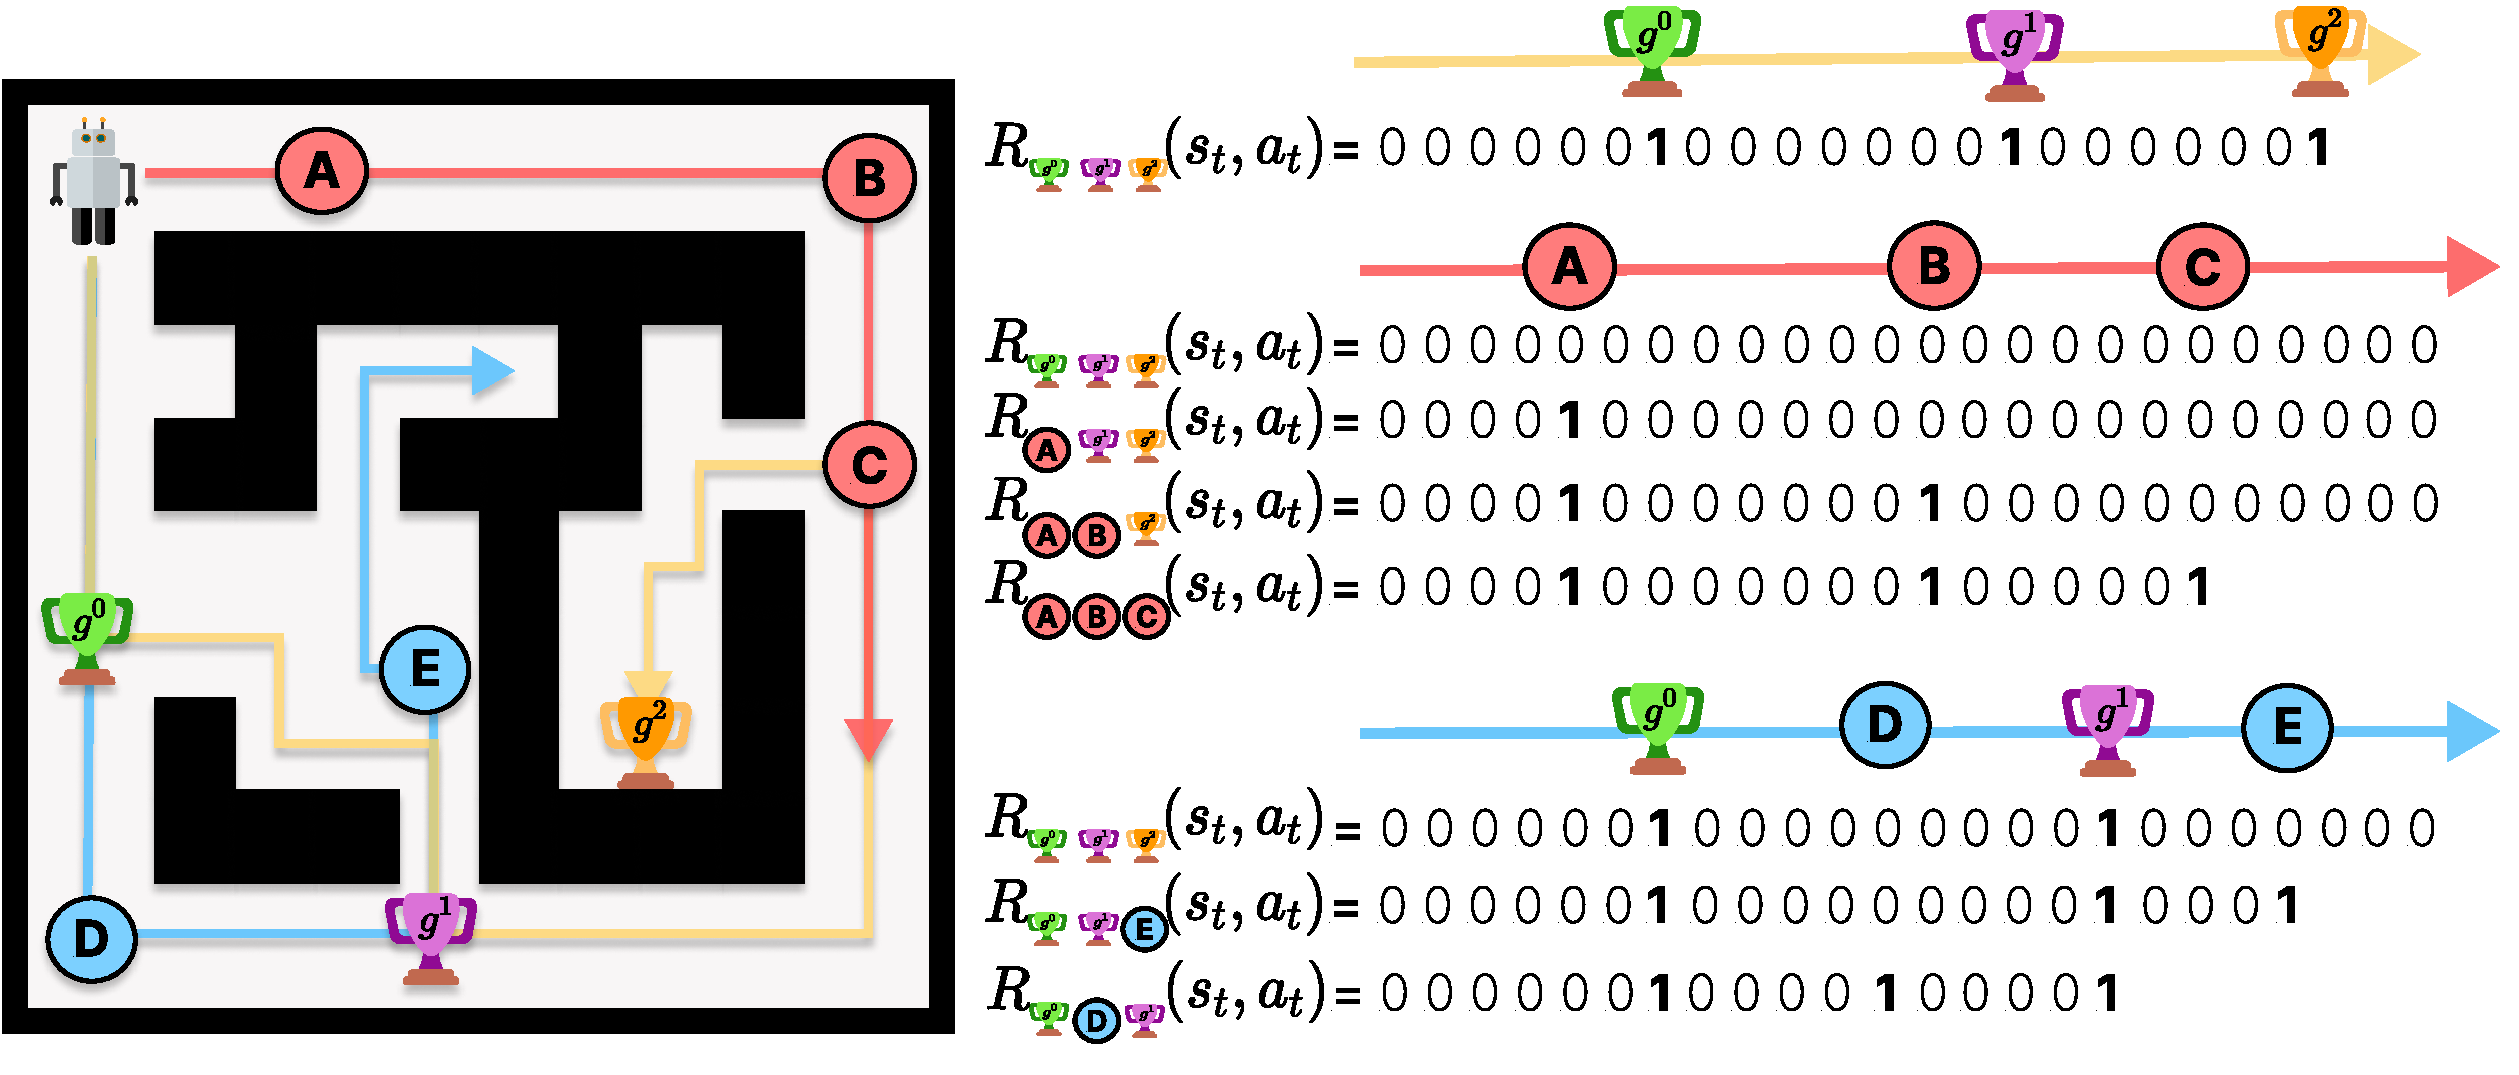
\includegraphics[width=.68\textwidth]{figs/relabel_new_colors.pdf}}
\vspace{-2mm}
\end{figure}

Our relabeling scheme works in two steps. First, we do not restrict goals to represent target states and allow them to be an abstract set of tokens or strings from a closed vocabulary. During rollouts, we can evaluate the goal tokens we were instructed to achieve and record alternatives that can be used for relabeling. The second step extends the HER relabeling scheme to ``instructions'', or sequences of up to $k$ subgoals. If an agent is tasked with $k$ goals but only completes the first $n \leq k$ steps of the instruction, we sample $h \in [0, k-n]$ timesteps that provide alternative goals, and then sample from all the goals achieved at those timesteps. We merge the $h$ alternative goals into the original instruction in chronological order and replay the trajectory from the beginning, recomputing the reward for the new instruction, which leads to a return of $n + h$ when rewards are binary. Figure \ref{fig:relabel} illustrates the technique with a maze-navigation example. Our implementation also considers importance-sampling variants that weight goal selection based on rarity and improve sample efficiency. Details are discussed in Appendix \ref{app:importance_sampling}.